\documentclass[border=5pt]{standalone}
\usepackage{tikz}
\usepackage{pgfplots}
\pgfplotsset{compat=1.18}
\usetikzlibrary{intersections}
\usetikzlibrary{math}
\usetikzlibrary{positioning}
\begin{document}
    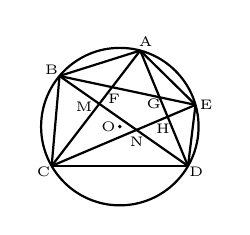
\begin{tikzpicture}
        \draw[thick] (0,0) circle (1);
        \coordinate (A) at (75:1);
        \coordinate (B) at (140:1);
        \coordinate (C) at (210:1);
        \coordinate (D) at (330:1);
        \coordinate (E) at (16:1);
        \coordinate (O) at (0,0);
        \fill[black] (A) circle (0.005) node[above right =-2pt and -4pt]{\tiny A};
        \fill[black] (B) circle (0.005) node[above left=-3pt and -3pt] {\tiny B };
        \fill[black] (C) circle (0.005) node[below left=-3pt and -3pt] {\tiny C };
        \fill[black] (D) circle (0.005) node[below right=-3pt and -3pt] {\tiny D };
        \fill[black] (E) circle (0.005)node[right=-2pt] {\tiny E };
        \fill[black] (O) circle (0.025) node[left=-2pt] {\tiny O};
        \draw[thick] (A) -- (B);
        \draw[thick] (B) -- (C);
        \draw[thick] (C) -- (D);
        \draw[thick] (A) -- (E);
        \draw[thick] (D) -- (E);
        \draw[thick, name path=AC] (A) -- (C);
        \draw[thick, name path=AD] (A) -- (D);
        \draw[thick, name path=BD] (B) -- (D);
        \draw[thick, name path=BE] (B) -- (E);
        \draw[thick, name path=CE] (C) -- (E);
        \path[name intersections={of=AC and BD, by = M}];
        \path[name intersections={of=CE and BD, by = N}];
        \path[name intersections={of=BE and AC, by = F}];
        \path[name intersections={of=CE and AD, by = H}];
        \path[name intersections={of=BE and AD, by = G}];
        \fill[black] (M) circle (0.005) node[below left=-4pt and -1pt] {\tiny M};
        \fill[black] (F) circle (0.005) node[below right=-1pt and -5pt] {\tiny F};
        \fill[black] (G) circle (0.005) node[below left=-3pt and -4pt] {\tiny G};
        \fill[black] (N) circle (0.005) node[below =-1pt] {\tiny N};
        \fill[black] (H) circle (0.005) node[below left = -1pt and -4.3pt] {\tiny H};
    \end{tikzpicture}
\end{document}